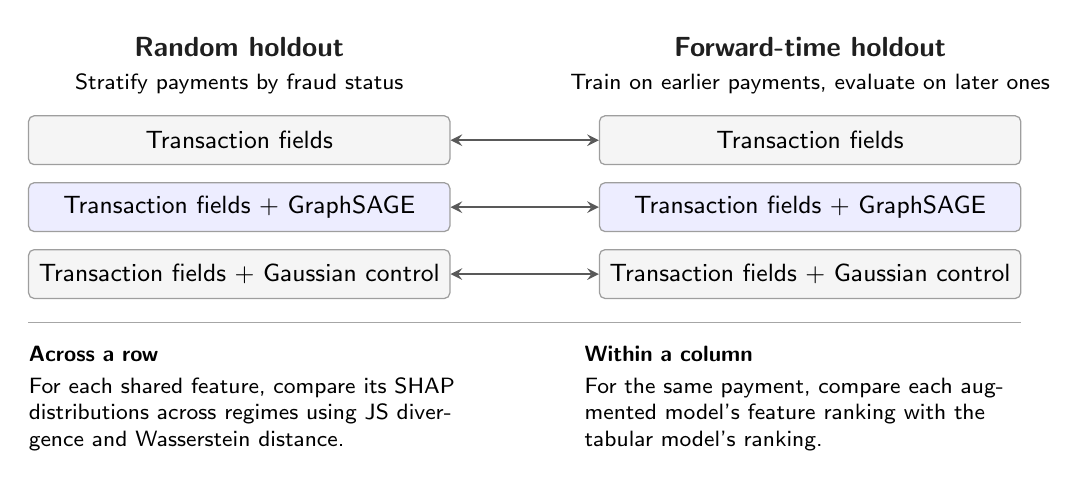
\begin{tikzpicture}[x=1cm,y=1cm,font=\sffamily\small,
  cell/.style={rounded corners=2pt,draw=black!38,line width=.45pt,
               minimum width=5.35cm,minimum height=.62cm,inner sep=2pt},
  columnhead/.style={font=\sffamily\bfseries,align=center,text=black!88},
  link/.style={<->,>=stealth,line width=.85pt,draw=black!65}]
  \node[columnhead] at (0,0) {Random holdout};
  \node[columnhead] at (7.25,0) {Forward-time holdout};
  \node[font=\sffamily\footnotesize] at (0,-.48) {Stratify payments by fraud status};
  \node[font=\sffamily\footnotesize] at (7.25,-.48) {Train on earlier payments, evaluate on later ones};

  \foreach \y/\name/\fillcolor in {
    -1.19/Transaction fields/black!4,
    -2.04/Transaction fields + GraphSAGE/blue!7,
    -2.89/Transaction fields + Gaussian control/black!4}{
    \node[cell,fill=\fillcolor] (left) at (0,\y) {\name};
    \node[cell,fill=\fillcolor] (right) at (7.25,\y) {\name};
    \draw[link] (left.east) -- (right.west);
  }
  \draw[black!35] (-2.68,-3.50) -- (9.93,-3.50);
  \node[anchor=north west,inner sep=0pt,text width=5.66cm,align=left,
        font=\sffamily\footnotesize] at (-2.68,-3.80)
     {\textbf{Across a row}\\[2pt]For each shared feature, compare its SHAP distributions across regimes using JS divergence and Wasserstein distance.};
  \node[anchor=north west,inner sep=0pt,text width=5.55cm,align=left,
        font=\sffamily\footnotesize] at (4.38,-3.80)
     {\textbf{Within a column}\\[2pt]For the same payment, compare each augmented model's feature ranking with the tabular model's ranking.};
\end{tikzpicture}
